\begin{figure}[H]
	\centering
	\begin{tabular}{p{1.5in} p{1.5in} p{1.5in}} 
	  \hline \\[.5em]
	  % algorithms
	  \docslink{maze_dataset.html\#LatticeMaze.as_ascii}{\texttt{as\_ascii()}}
	  & \docslink{maze_dataset.html\#LatticeMaze.as_pixels}{\texttt{as\_pixels()}}
	  & \docslink{maze_dataset/plotting.html\#MazePlot}{\texttt{MazePlot()}} \\[.5em]
	  % descriptions
		Simple text format for displaying mazes, useful for debugging in a terminal environment.
		& NumPy array of \texttt{dtype=uint8} and shape \texttt{(height, width, 3)}. The last dimension is RGB color.
		& Feature-rich plotting utility with support for multiple paths, heatmaps over positions, and more. \\[1em]
	  \hline \\
	  % examples
		\multicolumn{1}{l}{
		  \hspace{-1.5em}\raisebox{0.85\height}{
			  {
% \footnotesize
\ttfamily
\setlength{\tabcolsep}{0.3em}
\renewcommand{\arraystretch}{0.75}
\begin{tabular}{ccccccccccc}
\# & \# & \# & \# & \# & \# & \# & \# & \# & \# & \# \\
\# &   &   &   &   & \textcolor{blue}{X} & \textcolor{blue}{X} & \textcolor{blue}{X} & \# &  & \# \\
\# &   & \# & \# & \# & \textcolor{blue}{X} & \# & \textcolor{blue}{X} & \# &   & \# \\
\# &   &   &   & \# & \textcolor{blue}{X} & \# & \textcolor{green}{S} &   &   & \# \\
\# & \# & \# & \# & \# & \textcolor{b			lue}{X} & \# & \# & \# & \# & \# \\
\# & \textcolor{blue}{X} & \textcolor{blue}{X} & \textcolor{blue}{X} & \textcolor{blue}{X} & \textcolor{blue}{X} & \# & \textcolor{red}{E} & \textcolor{blue}{X} & \textcolor{blue}{X} & \# \\
\# & \textcolor{blue}{X} & \# & \# & \# &   & \# & \# & \# & \textcolor{blue}{X} & \# \\
\# & \textcolor{blue}{X} & \# &   &   &   &   &   & \# & \textcolor{blue}{X} & \# \\
\# & \textcolor{blue}{X} & \# & \# & \# & \# & \# & \# & \# & \textcolor{blue}{X} & \# \\
\# & \textcolor{blue}{X} & \textcolor{blue}{X} & \textcolor{blue}{X} & \textcolor{blue}{X} & \textcolor{blue}{X} & \textcolor{blue}{X} & \textcolor{blue}{X} & \textcolor{blue}{X} & \textcolor{blue}{X} & \# \\
\# & \# & \# & \# & \# & \# & \# & \# & \# & \# & \#
\end{tabular}
}
		  }
		}
		% 	\begin{minipage}[b]{1.6in}
		%   \setlength{\baselineskip}{0.9em}
		% 	\end{minipage}
		& \multicolumn{1}{c}{
		  
\includegraphics[width=0.25\textwidth]{figures/outputs-pixels.pdf}
		}
		& \multicolumn{1}{r}{
		  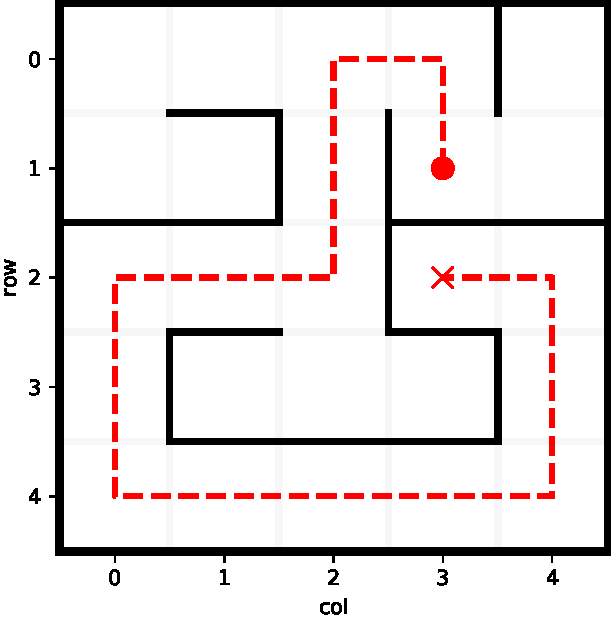
\includegraphics[width=0.27\textwidth, trim={0 0.8cm -.3cm, -.5cm}, clip]{figures/outputs-mazeplot.pdf}
		} \\[1em]
	  
	  \hline \\
	\end{tabular}
	\caption{Various output formats. Top row (left to right): ASCII diagram, rasterized pixel grid, and advanced display tool.}
	\label{fig:output-fmts}
\end{figure}